\part{Classification automatique des activités cérébrales} % (fold)
\label{prt:classification_ _automatique_ _des_ _activités_ _cérébrales_}
	\section{Schéma Général} % (fold)
	cf~\ref{fig_orga}, page~\pageref{fig_orga}.
		\label{sec:schéma_générale}
		\begin{figure}[t]
			\centering
			    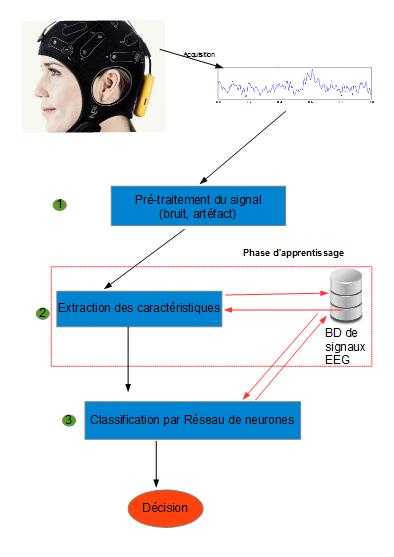
\includegraphics{../organigramme/orga.jpg} \\
		    	\captionof{figure}{Organigramme du fonctionnement générale de l'application}
				\label{fig_orga}
			\end{figure}

	\section{Pré-Traitement du signal} % (fold)
	\label{sec:pré_traitement_du_signal}
Cette étape consiste en un traitement sur le signal EEG obtenu afin de réduire les "bruits"(ou artefact) crées par les activités du sujet lors de l’acquisition du signal, telles: la position du sujet(sachant que un EEG standard se fait en position allongée ou assise avec un sujet relaxé), les mouvements des muscles du visage (exemple: clignement des yeux). Ainsi on applique une transformée de Fourrier au signal afin d'éliminer les bruits .
	
	% section pré_traitement_du_signal (end)
	\section{Extraction des caractéristiques} % (fold)
	\label{sec:extraction_des_caractéristiques}
	Cette étape est très importante car elle permet de déduire des caractéristiques notables du signal, elle se déroule lors de la phase d'apprentissage du réseau de neurones. Ainsi, un signal sera caractérisé par un vecteur de caractéristiques. On peut déduire plusieurs types de caractéristiques : temporelles, fréquentielles, tempo-fréquentielles.

	% section extraction_des_caractéristiques (end)
	\section{Classification par réseaux de neurones} % (fold)
	\label{sec:classification_par_réseaux_de_neurones}
	Pour la prise de décision nous avons choisi d'utiliser un réseau de neurones SOM, ainsi le signal sera classifié selon différents types de classes. Ces classes seront les activités du sujet que l'on veut détecter. 
	% section classification_par_réseaux_de_neurones (end)
	% section schéma_générale (end)
% part classification_ _automatique_ _des_ _activités_ _cérébrales_ (end)